\documentclass{article}
\usepackage[slovene]{babel}
\usepackage[utf8]{inputenc}
\usepackage[T1]{fontenc}
\usepackage{lmodern}
\usepackage{hyperref}
\usepackage{amsmath}
\usepackage{amsthm}
\usepackage{enumitem}
\usepackage{amssymb}
\usepackage{graphicx}
\usepackage{float}


\newtheorem{definition}{Definicija}[section] 
\newtheorem{theorem1}{Trditev}[section]
\newtheorem{lemma}{Lema}[section]

\title{Projektna naloga iz statistike}
\author{Martin Žust}
\date{2. 1. 2024}

\begin{document}

\section{Analiza prebivalcev mesta Kibergrad}

\subsection{Dohodki po četrtih}
V naši projektni nalogi nas je najprej zanimalo, kako se razlikujejo dohodki družin po četrtih. Opaziti smo želeli ali katera iz med četrti 
posebno izstopa v eno ali drugo smer. S tem namenom smo vzeli enaostavni slučajni vzorec velikosti 100 iz vsake četrti. V isti koordinatni sistem smo nato 
narisali škatlo z brki za vse štiri vzorce, kar je prikazano na sliki \ref{fig:slika1}.

\begin{figure}[H]
    \caption{Dohodki po četrtih}
    \centering
    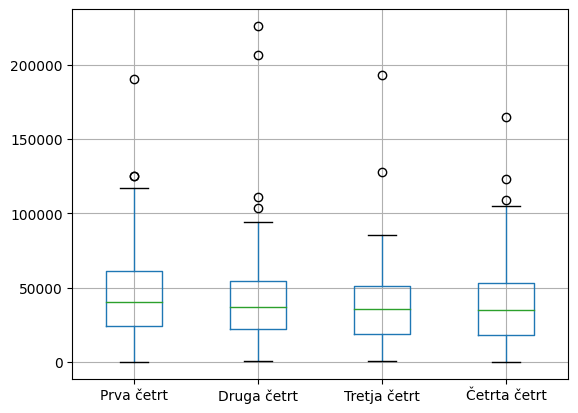
\includegraphics[scale=0.8]{dohodki_po_cetrtih.png}
    \label{fig:slika1}
\end{figure}

Iz slike \ref{fig:slika1} opazimo konkretne razlike med posameznimi četrtmi. Vendar bi lahko prišlo do napake zaradi premajhnih vzorcev. Po limitnih 
zakonih iz teorije verjetnosti namreč vemo, da večji vzorci dajejo večjo gotovost glede reprezentativnosti vzorca glede na celotno populacijo. S tem namenom 
vzamemo še štiri dodatne enostavne slučajne vzorce iz prve (severne) četrti enake velikosti kot prej. Škatle z brki za vseh pet izbranih slučajnih vzorcev iz severne 
četrti je prikazano na sliki \ref{fig:slika2}.

\begin{figure}[H]
    \caption{Slučajni vzorci v prvi četrti}
    \centering
    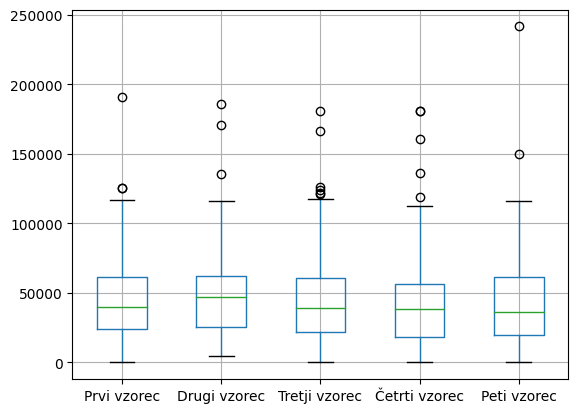
\includegraphics[scale=0.8]{vzorci_severne_cetrti.png}
    \label{fig:slika2}
\end{figure}

Opazimo, da se škatle z brki v prvi četrti med sabo ne razlikujejo nič manj kot škatle z brki po posameznih četrtih. Zaključimo, da so vzorci, ki 
smo jih vzeli premajhni, da bi iz njih lahko potegnili smiselne zaključke. 

%Dodaj vzorce velikosti 2000. 

%Dodaj primerjavo varianc. 

\subsection{Indeks srečnosti}

Za prebivalce mesta Kibergrad definiramo indeks srečnosti družine. Srečnost družine sem definiral s pomočjo lastnega občutka. Tako sem se držal principa, da 
vsak otrok pripomore k dodatni sreči družine. Z drugimi besedami, srečnost družine je linearno odvisna od števila otrok, ki jih ima družina. Po drugi strani se mi zdi, da niti previsoka 
niti prenizka izobrazba nista dobri za človekovo srečo. Tako je faktor, ki ga prispeva izobrazba največji pri povprečni izobrazbi. Kot zadnje pa sem pri indeksu srečnosti upošteval tudi 
prihodek, ki ga ima družina. Večji dohodek pripomore k večji srečnosti, vendar ne linaerno. Pri dohokdu od 0 do povprečnega dohodka srečnost raste eksponentno z večanjem dohodka. Ko pa je dohodek 
večji od povprečnega, pa ta na srečnost vpliva logaritemsko. 

Definirajmo vse skupaj bolj matematično. Označimo z $otr(D)$ število otrok, ki jih ima družina $D$. Nadalje z $izo(D)$ označimo najvišjo izobrazbo družine $D$ in z $doh(D)$ letni 
dohodek družine. Za definicijo indeksa srečnosti $S(D)$ potrebujemo še dve funkciji. Prva je funkcija $f(x)$, ki opisuje vpliv dohodka na srečnost:
$$
f(x) =
\begin{cases}
    2^{x/\mu_{doh}}; & \text{če } x < \mu_{doh} \\
    2 + \log_2 (1 + \frac{x - \mu_{doh}}{\mu_{doh}}); & \text{če } x \geq \mu_{doh}
\end{cases}
$$ 
Pri tem $\mu_{doh}$ označuje poprečen letni dohodek v mestu Kibergrad. Graf te funkcije je prikazan na sliki \ref{fig:slika3}.

\begin{figure}[H]
    \caption{Funkcija $f(x)$ za faktor dohodka}
    \centering
    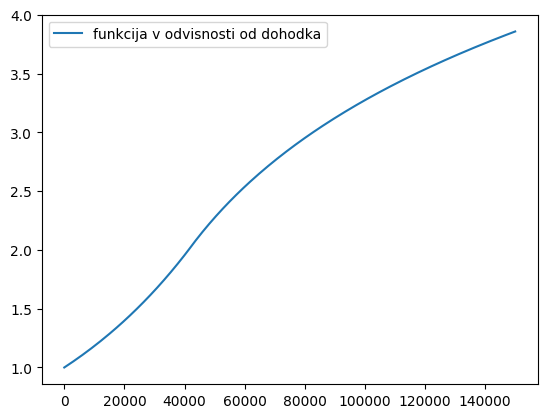
\includegraphics[scale=0.6]{funkcija_v_odvisnosti_od_dohodka.png}
    \label{fig:slika3}
\end{figure}

Druga pa je funkcija $g(x)$, ki opisuje vpliv izorazbe na srečnost. Definirana je kot gostota normalne porazdelitve:

$$
g(x) = \frac{1}{\sqrt{2 \pi \sigma_{izo}^2}} e^{-\frac{(x-\mu_{izo})^2}{2 \sigma_{izo}^2}}
$$
Pri tem je $\sigma_{izo}$ standardni odklon stopnje izobrazbe na podatkih mesta Kibergrad. Ko imamo definirani funkciji $f(x)$ in $g(x)$,
lahko definiramo indeks srečnosti:

$$
S(D) = otr(D) \cdot f(doh(D)) \cdot (g(izo(D)) + 20)
$$

Pri tej definiciji je veliko družin, katerih srečnost je 0, ker imajo 0 otrok. Dobimo porazdelitev srečnosti, ki je prikazana na histogramu \ref{fig:slika4}.

\begin{figure}[H]
    \caption{Histogram srečnosti v mestu Kibergrad}
    \centering 
    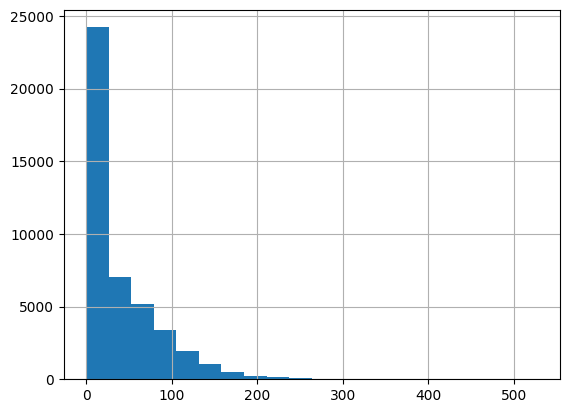
\includegraphics[scale=0.8]{histogram_srecnosti.png}
    \label{fig:slika4}
\end{figure}

Zanimala bi nas tudi srečnost v odvisnosti od dohodka. V tem primeru dobimo graf na sliki \ref{fig:slika5}.

\begin{figure}[H]
    \caption{Srečnost v odvisnosti od dohodka}
    \centering
    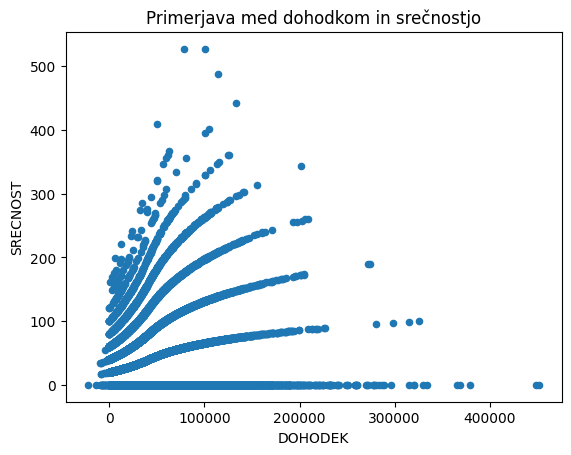
\includegraphics[scale=0.6]{dohodek_in_srecnost.png}
    \label{fig:slika5}
\end{figure}

Opazimo močno izračene razrede oziroma krivulje. Vsaka krivulja predstavlja razred za število 
otrok in je oblike grafa funkcije $f(x)$. 

\end{document}